\chapter{Introduction and Problem Formulation}
\label{ch:ch01_introduction}

% --- Merged from ch01_introduction.tex ---

\section{Introduction}
\label{ch:introduction}

Physical AI controllers---battery dispatch optimisers, autonomous-vehicle
planners, robotic manipulators---share a structural assumption so pervasive
that it is rarely stated explicitly: \emph{the observation available to the
controller faithfully represents the physical state of the plant.}  This
dissertation investigates what happens when that assumption fails, using
grid-scale battery energy storage systems (BESS) as the first rigorous
validation surface.

\subsection{The Hidden Assumption in Physical AI}

Every feedback controller closes a loop: sense the plant state, compute an
action, actuate, repeat.  Classical control theory formalises this loop with
a state vector~$x_t \in \mathcal{X}$, a measurement function~$h$, and an
observation~$y_t = h(x_t) + v_t$, where $v_t$ is zero-mean sensor noise.
When the noise is well-characterised---Gaussian, bounded, independent---the
Kalman filter or its nonlinear descendants recover the true state with known
error bounds, and the controller can act as if it sees the truth.

Modern cyber-physical systems (CPS) break this contract in ways that are
neither Gaussian nor bounded.  Telemetry arrives over packet-switched
networks subject to dropout, delay, replay, and stale-sensor failure.
The resulting observation~$\hat{x}_t$ is not simply $x_t$ plus noise;
it may be \emph{structurally incorrect}: the controller sees a state that
the plant never occupied.  No amount of Kalman filtering can correct for a
reading that was dropped entirely and replaced by an interpolated hold.

The consequence is subtle but dangerous.  The controller evaluates its
safety constraints against $\hat{x}_t$, not $x_t$.  If $\hat{x}_t$
satisfies the constraints, the controller judges the situation safe.
Meanwhile, the true state~$x_t$ may already violate a physical limit.
The system is \emph{observationally safe} but \emph{physically unsafe}---a
condition we call the \emph{Observation-Action Safety Gap} (OASG).

\subsection{Why Observed Safety Can Differ from Physical Safety}

Consider a battery dispatched at 50\% SOC (state of charge).  A telemetry
packet carrying the latest voltage and current readings is delayed by two
intervals.  The controller still sees SOC~$= 50\%$ and issues a large
discharge.  In reality, a prior discharge already pushed SOC to 22\%.
The new action drives the physical SOC below the 20\% safety floor.
The observed trajectory shows no violation; the true trajectory shows a
hard constraint breach.  Figure~\ref{fig:oasg-hero} illustrates this
gap and the five-stage DC3S pipeline that closes it.

\begin{figure}[htbp]
\centering
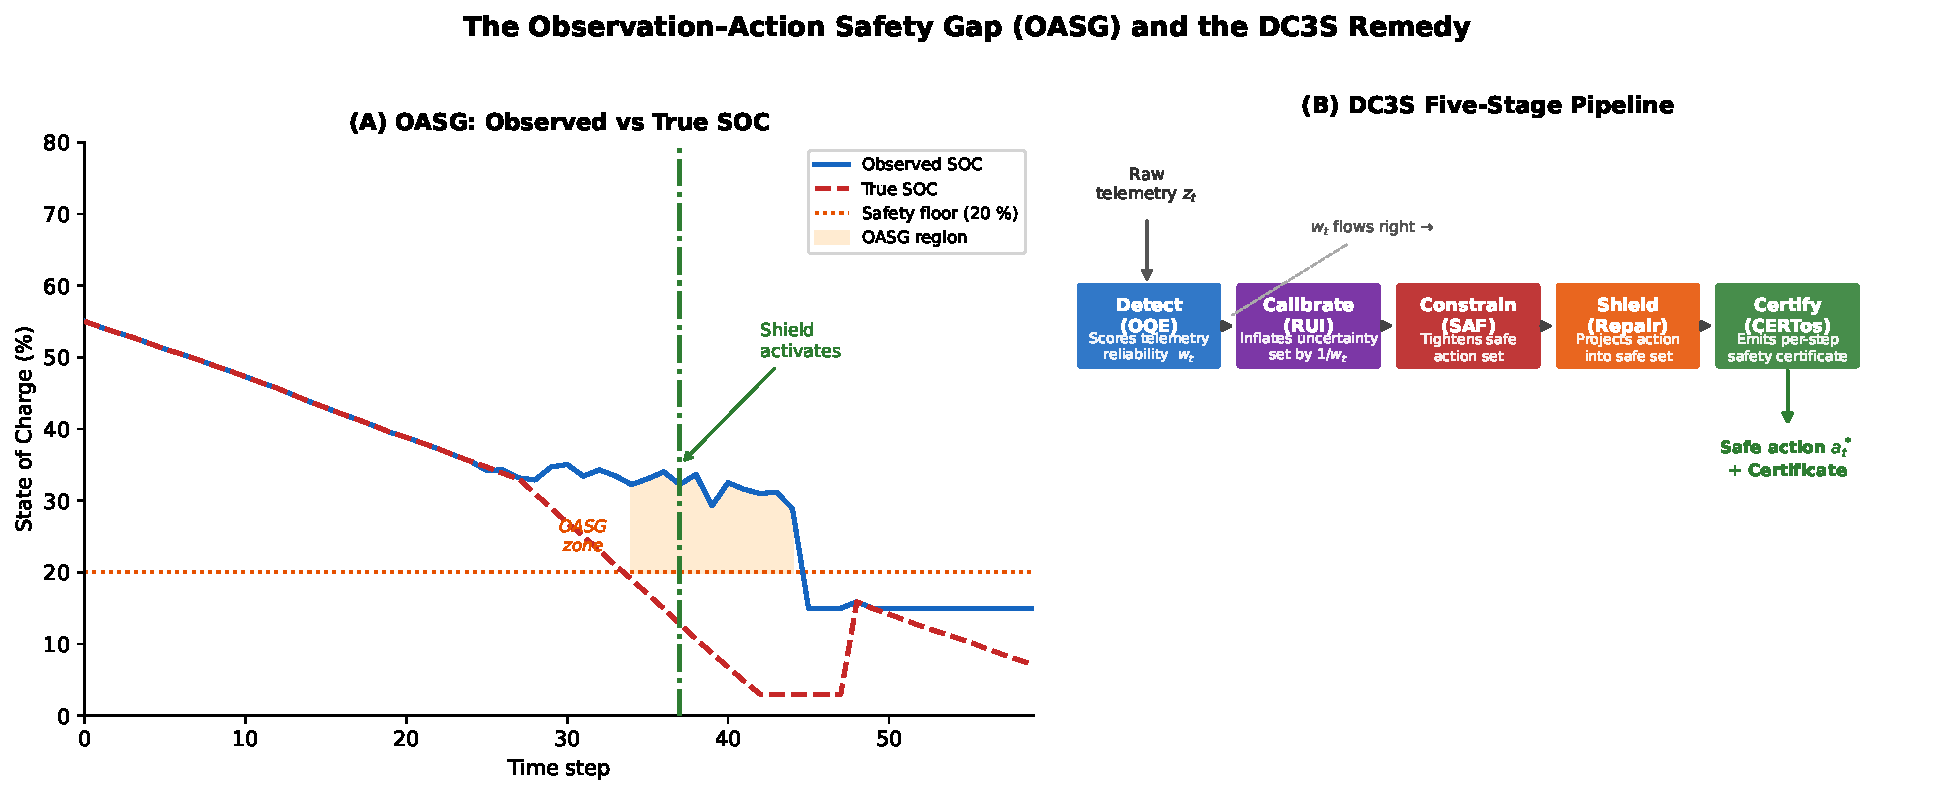
\includegraphics[width=0.95\linewidth]{paper/assets/figures/fig_oasg_hero}
\caption{The OASG in practice (left): observed SOC appears above the 20\%
safety floor while the true SOC has already breached it.  DC3S detects
reliability degradation, inflates the safety margin, and intercepts the
unsafe action before dispatch.  The DC3S five-stage pipeline (right)
maps the live OQE reliability score $w_t$ through calibrated uncertainty
inflation (RUI), tightened action constraints (SAF), safe-action repair,
and auditable runtime certificates (CERTos).}
\label{fig:oasg-hero}
\end{figure}

This is not a contrived edge case.  Field telemetry from US-grid EIA-930
data exhibits dropout rates of 5--15\% under normal operation and exceeding
30\% during storm events.  Germany's ENTSO-E feeds show comparable
patterns with additional regulatory delay.  Every dropped, delayed, or
stale reading widens the gap between observation and truth.

\subsection{The Observation-Action Safety Gap}
\label{sec:intro-oasg}

We define the OASG as the divergence between a controller's safety
assessment on its observed state and the actual safety status of the
physical plant:

\begin{definition}[Observation-Action Safety Gap (OASG)]
\label{def:oasg-informal}
Let $\hat{x}_t$ be the controller's observation and $x_t$ the true
state.  The \emph{OASG} at time~$t$ is the event
\[
  \mathcal{G}_t \;=\;
  \bigl\{\,a_t \in \mathcal{A}(\hat{x}_t)\;\bigr\}
  \;\cap\;
  \bigl\{\,a_t \notin \mathcal{A}(x_t)\;\bigr\},
\]
where $\mathcal{A}(x)$ denotes the set of actions satisfying all safety
constraints at state~$x$.  When $\mathcal{G}_t$ is non-empty, the
controller has chosen an action that appears safe on the observation
but violates constraints on the truth.
\end{definition}

The OASG is \emph{invisible} to any evaluation protocol that checks
constraints only on the observed trajectory.  Revealing it requires
maintaining a parallel \emph{true-state trajectory}---a dual-trajectory
architecture that is a cornerstone of the CPSBench harness developed in
this work (Chapter~\ref{ch:safety-illusion}).

\subsection{Why the Battery Domain Exposed the Problem First}

Batteries present three properties that make the OASG both acute and
measurable:

\begin{enumerate}
  \item \textbf{Hard state constraints.}  SOC must remain within
    $[\text{SOC}_{\min}, \text{SOC}_{\max}]$.  There is no elastic zone;
    violating the lower bound risks cell damage, and violating the upper
    bound risks thermal runaway.
  \item \textbf{High action-to-state sensitivity.}  A single dispatch
    decision at 50~MW for a 100~MWh battery moves SOC by 50\% in one hour.
    Even a brief observation error translates into a large true-state
    deviation.
  \item \textbf{Network-mediated telemetry.}  Grid-scale batteries are
    monitored via SCADA, cellular, or satellite links---all subject to the
    packet-level faults that create the OASG.
\end{enumerate}

Other CPS domains (autonomous vehicles, industrial robots) share
property~(3) but lack the clean measurability of~(1) and~(2).  The battery
domain is therefore the ideal \emph{first proving ground} for a general
theory of observation-aware safety.

\subsection{The ORIUS Principle}
\label{sec:orius-principle}

ORIUS---\textbf{O}bservation-\textbf{R}eliability--aware
\textbf{U}ncertainty-\textbf{I}nflated \textbf{S}afety---is the
organising principle of this dissertation.  It prescribes a four-stage
runtime pipeline:

\begin{enumerate}
  \item \textbf{Observation Quality Engine (OQE).}  Score the current
    telemetry reliability $w_t \in [w_{\min}, 1]$ using delay, freshness,
    spike, and stale-sensor features.
  \item \textbf{Reliability-aware Uncertainty Inflator (RUI).}  Inflate
    conformal prediction intervals by a factor proportional to $1/w_t$,
    widening the uncertainty set when observations are poor.
  \item \textbf{Safe-Action Filter (SAF).}  Tighten the feasible action
    set so that the dispatched action remains within SOC bounds even under
    worst-case realisations of the inflated uncertainty.
  \item \textbf{DC3S Shield.}  Issue a \emph{safety certificate} for
    every dispatched action, recording the observation quality, uncertainty
    bounds, and the margin to the nearest constraint.
\end{enumerate}

DC3S---the \textbf{D}ata-\textbf{C}entric \textbf{C}ertified
\textbf{C}onformal \textbf{S}hield---is the concrete realisation of the
ORIUS principle for the battery dispatch domain.

\subsection{Research Questions}

This dissertation addresses three central questions:

\begin{enumerate}
  \item[\textbf{RQ1.}] \emph{Does the Observation-Action Safety Gap exist
    in real-world battery dispatch?}  Specifically, do standard controllers
    (deterministic LP, robust MPC, stochastic risk-aware) produce actions
    that satisfy observed-state constraints while violating true-state
    constraints under realistic telemetry degradation?
  \item[\textbf{RQ2.}] \emph{Can a certificate-aware runtime safety layer
    close the gap?}  Can a lightweight online shield, informed by
    observation quality scores and conformal uncertainty, guarantee
    physical safety at the cost of bounded economic intervention?
  \item[\textbf{RQ3.}] \emph{What is the formal safety guarantee, and
    under what assumptions does it hold?}  Can we state a theorem of the
    form ``if telemetry faults satisfy bounds~$\mathcal{F}$ and the
    calibration set is exchangeable, then the true-state violation rate is
    at most~$\alpha$ with probability at least~$1 - \delta$''?
\end{enumerate}

\subsection{Contributions}

The principal contributions are:

\begin{enumerate}
  \item \textbf{Formalisation of the OASG.}  A rigorous definition of the
    gap between observed-state and true-state safety, together with a
    taxonomy of telemetry faults that create it
    (Chapter~\ref{ch:problem-formulation}).
  \item \textbf{The DC3S runtime shield.}  A four-stage pipeline (OQE,
    RUI, SAF, Shield) that closes the OASG with a provable coverage
    guarantee (Chapters~\ref{ch:safety-illusion}--\ref{ch:cert-half-life-blackout}).
  \item \textbf{CPSBench evaluation harness.}  A deterministic,
    dual-trajectory benchmark for battery dispatch under telemetry faults,
    enabling reproducible comparison of observation-aware controllers
    (Chapter~\ref{ch:orius-bench-battery}).
  \item \textbf{Empirical validation on US and DE grids.}  End-to-end
    experiments on EIA-930 (US) and ENTSO-E (Germany) data demonstrating
    zero true-state SOC violations across all tested dropout rates, with
    intervention rates below 20\%.
  \item \textbf{Extension results.}  Certificate half-life analysis
    (Chapter~\ref{ch:cert-half-life-blackout}), graceful degradation
    (Chapter~\ref{ch:graceful-degradation}), compositional fleet safety
    (Chapter~\ref{ch:compositional-safety-fleets}), and a CertOS runtime
    chapter that promotes the certificate lifecycle from roadmap language
    into bounded systems evidence (Chapter~\ref{ch:certos-runtime}).
\end{enumerate}

\subsection{Contribution Boundary}

This work does \emph{not} claim to solve the general partial-observability
problem for all CPS domains.  The safety guarantee is stated and validated
for the battery dispatch domain under the fault model of
Chapter~\ref{ch:problem-formulation}.  Extension to other domains
(e.g., autonomous driving, surgical robotics) requires domain-specific
instantiation of the OQE and SAF stages and is left to future work.

We also do not replace the upstream forecast or optimisation model.  DC3S
is a \emph{post-optimiser safety layer}: it takes the dispatch action
produced by any optimiser and certifies or corrects it before actuation.
The economic optimiser remains a black box to the shield.

\subsection{Scope and Limitations of the Safety Guarantees}

The main ORIUS theorem statements are marginal coverage guarantees.  They
bound aggregate true-state risk over the deployment distribution induced by
observations, telemetry faults, and calibration residuals.  They do not claim
conditional coverage for every specific observation and fault realization.

That boundary is deliberate.  Conditional coverage is not achievable in full
generality under arbitrary non-exchangeable distributions, so the thesis keeps
the flagship results at the strongest level that can be defended on the active
artifact surface: finite-sample marginal coverage.  Later grouped analyses,
including reliability-bin and Mondrian-style evaluations, refine that
guarantee for explicit subpopulations but do not upgrade the core claim into a
universal per-step worst-case statement.

\subsection{Relationship to Prior Work}

This dissertation supersedes the earlier battery-first ORIUS monograph and its
associated frozen release bundles.  The earlier package established the
battery reference surface, the original theorem ladder, and the core
calibration and drift-monitoring workflow.  Those battery results are retained
here as the deepest theorem-to-artifact witness rather than being renumbered
or discarded.

The present thesis extends that prior work in four ways.  First, it isolates a
domain-agnostic repair-and-certify kernel instead of leaving the argument
battery-local.  Second, it widens the empirical program into a tiered
cross-domain package while preserving explicit evidence boundaries for rows
that have not yet reached parity.  Third, it adds the later necessity,
lower-bound, and transfer results that clarify what the battery witness does
and does not imply beyond its home domain.  Fourth, it promotes certificate
lifecycle and release-manifest governance from appendicial audit material into
a first-class runtime object through CertOS and the claim-lock discipline.

\subsection{Organisation of the Manuscript}

The remainder of this dissertation is organised as follows:

\begin{description}
  \item[Chapter~\ref{ch:related-work}] surveys background and related work
    in battery dispatch, telemetry faults, conformal prediction, and
    runtime safety shields.
  \item[Chapter~\ref{ch:problem-formulation}] formalises the system model,
    fault model, SOC dynamics, the observation quality engine, and states
    the research questions mathematically.
  \item[Chapter~\ref{ch:safety-illusion}] defines the observed-state
    safety illusion and motivates the dual-trajectory evaluation paradigm.
  \item[Chapters~\ref{ch:assumptions}--\ref{ch:ablations}] develop the DC3S pipeline components, prove the
    coverage theorem, and present ablation studies.
  \item[Chapters~\ref{ch:cert-half-life-blackout}--\ref{ch:certos-runtime}]
    extend the framework to certificate temporal validity, graceful
    degradation, fleet composition, and certificate-aware runtime control.
  \item[Chapter~\ref{ch:orius-bench-battery}] describes the ORIUS-Bench
    battery track for reproducible benchmarking.
  \item[Chapter~\ref{ch:outside-current-evidence}] records bounded but
    intentionally non-promoted evidence surfaces, including the active
    probing audit and other claims that remain outside the defended core.
\end{description}


% --- Merged from ch03_problem_formulation.tex ---

\section{Problem Formulation}
\label{ch:problem-formulation}
\label{ch:formal-problem-formulation}

This chapter formalises the system model, telemetry fault model, battery
dynamics, and safety constraints that underpin the ORIUS framework.  We
state the research questions mathematically and delineate the scope
boundary of the dissertation.

\subsection{ORIUS System Context}
\label{sec:orius-context}

ORIUS is a renewable-aware battery dispatch platform that operates at
the \emph{optimise-to-dispatch boundary}: an upstream forecast-and-optimise
pipeline produces a candidate dispatch action~$a_t^{\star}$, and a
downstream safety layer either certifies or corrects the action before it
reaches the physical plant.  The system architecture comprises:

\begin{enumerate}
  \item \textbf{Forecast stage.}  CQR models predict load, solar, and
    wind trajectories over a configurable horizon, producing both point
    forecasts and conformal prediction intervals.
  \item \textbf{Optimise stage.}  A deterministic LP (or a pluggable
    alternative) maximises arbitrage revenue subject to SOC, power, and
    ramp constraints evaluated on the \emph{observed} state.
  \item \textbf{Dispatch stage (DC3S).}  The safety layer scores
    observation quality, inflates uncertainty, tightens action bounds, and
    issues a safety certificate for the final dispatched action.
\end{enumerate}

The boundary between stages~2 and~3 is the \emph{optimise-to-dispatch
boundary}.  Everything upstream of this boundary operates on the observed
state~$\hat{x}_t$; the safety layer's task is to ensure that the
dispatched action is safe on the \emph{true} state~$x_t$ despite the gap
between the two.

\subsection{ORIUS-MDP Formalisation}

\begin{definition}[ORIUS-MDP]
\label{def:orius-mdp-merged}
An ORIUS deployment is modelled as the 11-tuple
\[
  (\mathcal{S}, \mathcal{O}, \mathcal{W}, \mathcal{A}, \mathcal{C},
   \mathcal{T}, \mathcal{H}, \Omega, \mathcal{R}, \gamma, \mu_0),
\]
where $\mathcal{S}$ is the true-state space, $\mathcal{O}$ the observation
space, $\mathcal{W}=[w_{\min},1]$ the observation-quality space,
$\mathcal{A}$ the action space, and $\mathcal{C}\subsetneq\mathcal{S}$ the
closed safety set.  The true transition kernel is
$\mathcal{T}: \mathcal{S}\times\mathcal{A}\to\Delta(\mathcal{S})$, the
observation kernel is $\mathcal{H}: \mathcal{S}\to\Delta(\mathcal{O})$, the
quality map is $\Omega: Z^k\to\mathcal{W}$, the reward is
$\mathcal{R}: \mathcal{S}\times\mathcal{A}\to\mathbb{R}$, $\gamma\in[0,1)$ is
the discount factor, and $\mu_0$ is the initial-state distribution.

At runtime, the controller receives $(o_t,w_t)$ where
$o_t\sim\mathcal{H}(x_t)$ and $w_t=\Omega(z_{t-k+1:t})$ is computed
deterministically from the telemetry history.  Reliability-aware policies
therefore take the form $\pi:\mathcal{O}\times\mathcal{W}\to\Delta(\mathcal{A})$,
whereas quality-ignorant policies are restricted to
$\bar{\pi}:\mathcal{O}\to\Delta(\mathcal{A})$.
\end{definition}

\begin{remark}
The ORIUS-MDP differs from a classical POMDP not because observation is
partial, but because observation quality itself is exposed as a runtime state
component that conditions repair, fallback, and certification.  Safety is
always measured on the true-state trajectory rather than on the observation
trajectory.
\end{remark}

\subsection{The Hidden Safety Gap}
\label{sec:hidden-gap}

We now state the core safety problem in the battery domain.

\begin{definition}[Battery-domain OASG]
\label{def:battery-oasg}
Let $\mathrm{SOC}_t^{\mathrm{true}}$ denote the physical state of charge
and $\widehat{\mathrm{SOC}}_t$ the value available to the controller.
The \emph{battery-domain Observation-Action Safety Gap} at time~$t$ is the
event
\[
  \mathcal{G}_t^{\mathrm{bat}} \;=\;
  \Bigl\{\,a_t \in \mathcal{A}\!\bigl(\widehat{\mathrm{SOC}}_t\bigr)\Bigr\}
  \;\cap\;
  \Bigl\{\,a_t \notin \mathcal{A}\!\bigl(\mathrm{SOC}_t^{\mathrm{true}}\bigr)\Bigr\},
\]
where $\mathcal{A}(s)$ is the set of dispatch actions that keep the
subsequent SOC within the feasible range $[\mathrm{SOC}_{\min},
\mathrm{SOC}_{\max}]$.
\end{definition}

When $\mathcal{G}_t^{\mathrm{bat}}$ occurs, the controller has committed
a \emph{physically unsafe} action while believing it to be safe.

\subsection{State Objects and Telemetry Model}

\subsubsection{True State}

The true state at time~$t$ is the vector
\[
  x_t \;=\; \bigl(\mathrm{SOC}_t^{\mathrm{true}},\;
  L_t^{\mathrm{true}},\; S_t^{\mathrm{true}},\; W_t^{\mathrm{true}}\bigr)
  \;\in\; \mathcal{X} \subset \mathbb{R}^4,
\]
comprising the physical SOC and the true load, solar, and wind power at
the grid connection point.

\subsubsection{Observed State}

The observed state is the output of the telemetry channel:
\[
  \hat{x}_t \;=\; \mathcal{T}(x_t,\, \xi_t),
\]
where $\mathcal{T}$ is a (possibly stochastic) telemetry operator and
$\xi_t$ encodes the fault realisation at time~$t$ (dropout mask, delay
value, spike indicator, staleness flag).

\subsubsection{Observation Quality Score}
\label{sec:oqe-formula}

The Observation Quality Engine (OQE) computes a scalar reliability
score from the telemetry features:
\[
  w_t \;=\; \max\!\bigl(w_{\min},\;
    p_{\mathrm{miss},t} \cdot p_{\mathrm{delay},t}
    \cdot p_{\mathrm{ooo},t} \cdot p_{\mathrm{spike},t}\bigr),
\]
where each penalty factor $p_{\cdot} \in [0, 1]$ reflects a specific
fault channel:

\begin{description}
  \item[$p_{\mathrm{miss},t}$:] Fraction of expected readings that
    arrived in the current window.  Full reception yields $p_{\mathrm{miss}} = 1$;
    complete dropout yields $p_{\mathrm{miss}} = 0$.
  \item[$p_{\mathrm{delay},t}$:] Penalty for readings whose timestamp
    exceeds the freshness threshold: $p_{\mathrm{delay}} =
    \exp(-\lambda_d \cdot \bar{\tau}_t)$, where $\bar{\tau}_t$ is the
    mean delay in the window and $\lambda_d$ is a configurable decay rate.
  \item[$p_{\mathrm{ooo},t}$:] Fraction of readings arriving in
    chronological order.  Out-of-order arrivals indicate network jitter
    or replay.
  \item[$p_{\mathrm{spike},t}$:] Penalty for readings flagged as
    transient spikes: $p_{\mathrm{spike}} = 1 - n_{\mathrm{spike}} /
    n_{\mathrm{total}}$.
\end{description}

The floor $w_{\min} > 0$ ensures that the uncertainty inflator always
produces a finite interval; the default value is $w_{\min} = 0.05$.

\subsection{Fault Model}
\label{sec:fault-model}

We define the fault model as a tuple
$\mathcal{F} = (\rho, \bar{\tau}, \pi_s, \pi_{\mathrm{stale}}, \sigma_d)$:

\begin{itemize}
  \item $\rho \in [0, 1]$: dropout rate (probability that a packet is
    missing at any given step).
  \item $\bar{\tau} \ge 0$: mean packet delay in multiples of the
    decision interval $\Delta t$.
  \item $\pi_s \in [0, 1]$: probability that a reading is a transient
    spike.
  \item $\pi_{\mathrm{stale}} \in [0, 1]$: probability that a sensor
    output is frozen (stale).
  \item $\sigma_d > 0$: standard deviation of the covariate drift between
    calibration and deployment distributions.
\end{itemize}

The CPSBench harness (Chapter~\ref{ch:orius-bench-battery}) instantiates
each fault channel independently and provides composite scenarios
(e.g., \texttt{drift\_combo}) that activate all channels simultaneously.

\subsection{Battery Dynamics and Feasible Action Set}
\label{sec:battery-dynamics}

\subsubsection{SOC Dynamics}

The true SOC evolves according to:
\begin{equation}
\label{eq:soc-dynamics}
  \mathrm{SOC}_{t+1}^{\mathrm{true}} \;=\;
  \mathrm{SOC}_t^{\mathrm{true}}
  \;+\; \frac{\eta_c\,[a_t]^{+} \;-\; [a_t]^{-}/\eta_d}{E_{\max}}
  \;\cdot\; \Delta t,
\end{equation}
where:
\begin{itemize}
  \item $a_t \in \mathbb{R}$ is the dispatch action (positive = charge,
    negative = discharge),
  \item $[a_t]^{+} = \max(a_t, 0)$ and $[a_t]^{-} = \max(-a_t, 0)$
    denote the charge and discharge components,
  \item $\eta_c, \eta_d \in (0, 1]$ are the charge and discharge
    round-trip efficiencies,
  \item $E_{\max}$ is the battery energy capacity (MWh), and
  \item $\Delta t$ is the decision interval (hours).
\end{itemize}

\subsubsection{Feasible Action Set}

Given a SOC value~$s$, the feasible action set is:
\begin{equation}
\label{eq:feasible-set}
  \mathcal{A}(s) \;=\; \Bigl\{\,a \in [-\bar{P},\, \bar{P}] \;:\;
  \mathrm{SOC}_{\min} \;\le\;
  s + \frac{\eta_c [a]^{+} - [a]^{-}/\eta_d}{E_{\max}} \cdot \Delta t
  \;\le\; \mathrm{SOC}_{\max}\Bigr\},
\end{equation}
where $\bar{P}$ is the rated power limit (MW) and
$[\mathrm{SOC}_{\min}, \mathrm{SOC}_{\max}]$ are the regulatory SOC
bounds (typically 20\%--80\% for grid-scale lithium-ion systems).

\subsection{Dispatch Objective}

The upstream optimiser maximises expected arbitrage revenue over a
rolling horizon~$H$:
\begin{equation}
\label{eq:dispatch-obj}
  \max_{a_t, \ldots, a_{t+H-1}} \;\sum_{\tau=t}^{t+H-1}
  \pi_\tau \cdot a_\tau \cdot \Delta t
  \quad \text{s.t.} \quad
  a_\tau \in \mathcal{A}\!\bigl(\widehat{\mathrm{SOC}}_\tau\bigr)
  \;\;\forall\, \tau,
\end{equation}
where $\pi_\tau$ is the electricity price at step~$\tau$.  Note that the
constraints are evaluated on the \emph{observed} SOC; the optimiser has
no access to the true state.  The DC3S safety layer post-processes the
solution to enforce constraints on the true state via uncertainty
inflation.

\subsection{The Calibration Gap Under Degradation}
\label{sec:calibration-gap}

Conformal prediction intervals are calibrated on a held-out calibration
set collected under nominal telemetry conditions.  When deployment
telemetry degrades, the residual distribution shifts:

\begin{enumerate}
  \item Dropout introduces a positive bias in the imputed SOC (stale
    holds tend to overestimate SOC during discharge and underestimate
    during charge).
  \item Delay increases the variance of the residual because the
    controller acts on outdated information.
  \item Covariate drift invalidates the exchangeability assumption that
    underpins the conformal guarantee.
\end{enumerate}

The RUI stage compensates by scaling the conformal half-width by
$1/w_t$:
\begin{equation}
\label{eq:rui-inflation}
  q_{\mathrm{eff},t} \;=\; \frac{q_{\alpha}}{w_t},
\end{equation}
where $q_{\alpha}$ is the nominal conformal quantile.  As $w_t$
decreases, the effective half-width grows, widening the uncertainty set
and tightening the safe-action filter.

\subsection{Baseline Policies}
\label{sec:baselines}

We compare DC3S against three baseline dispatch policies:

\begin{description}
  \item[Deterministic LP.]  Solves~\eqref{eq:dispatch-obj} directly on
    $\hat{x}_t$ with no uncertainty handling.
  \item[Robust MPC.]  Maintains a fixed uncertainty tube
    $[\hat{x}_t - \epsilon, \hat{x}_t + \epsilon]$ with hand-tuned
    margin~$\epsilon$.  The tube does not adapt to observation quality.
  \item[Stochastic risk-aware.]  Samples $N$ scenarios from historical
    forecast errors and enforces CVaR constraints.  The scenario
    distribution is not conditioned on telemetry quality.
\end{description}

All baselines operate on the observed state and do not maintain a
true-state trajectory.  Their safety performance is therefore evaluated
\emph{ex post} by the CPSBench dual-trajectory harness.

\subsection{Research Questions Formalised}
\label{sec:rqs-formal}

We restate the research questions of Chapter~\ref{ch:introduction} in
mathematical terms.

\begin{description}
  \item[\textbf{RQ1} (Existence of the OASG).]
    Under fault model $\mathcal{F}$ with dropout rate $\rho > 0$, does
    there exist a time step~$t$ such that the OASG
    event~$\mathcal{G}_t^{\mathrm{bat}}$ (Definition~\ref{def:battery-oasg})
    occurs for at least one baseline policy?
  \item[\textbf{RQ2} (Closing the gap).]
    Does DC3S achieve
    $\mathrm{TSVR} = \frac{1}{T}\sum_{t=1}^T
    \mathbf{1}[\mathcal{G}_t^{\mathrm{bat}}] = 0$
    for all tested fault configurations, and at what intervention
    rate~$\mathrm{IR}$?
  \item[\textbf{RQ3} (Formal guarantee).]
    Under the bounded battery-domain assumption set A1--A5 collected in
    Appendix~\ref{app:assumptions}, does the coverage
    inequality
    \[
      \Pr\!\bigl[\,\mathrm{SOC}_{t+1}^{\mathrm{true}}
      \in [\mathrm{SOC}_{\min}, \mathrm{SOC}_{\max}]\,\bigr]
      \;\ge\; 1 - \alpha
    \]
    hold for all $t$ under fault model $\mathcal{F}$?
\end{description}

\subsection{Scope Boundary}
\label{sec:scope}

The formal results in this dissertation are stated for the following
scope:

\begin{itemize}
  \item \textbf{Domain.}  Grid-scale lithium-ion battery energy storage
    (100~MWh / 50~MW reference plant).
  \item \textbf{Decision granularity.}  Hourly dispatch ($\Delta t = 1$~h).
  \item \textbf{Fault model.}  The five-channel model of
    Section~\ref{sec:fault-model}, with dropout rates up to $\rho = 0.40$.
  \item \textbf{Forecast horizon.}  Up to 48~hours (the maximum horizon
    evaluated in the 48-hour trace studies).
  \item \textbf{Plant model.}  Linear SOC dynamics~\eqref{eq:soc-dynamics}
    with constant efficiencies.  Degradation effects (capacity fade,
    resistance growth) are not modelled in the core pipeline but are
    examined in the extension chapters.
\end{itemize}

Results outside this scope (sub-hourly dispatch, non-lithium chemistries,
vehicle-to-grid applications) require re-calibration and are deferred to
future work.

\subsection{Dataset Scope}
\label{sec:dataset-scope}

All experiments use two public data sources:

\begin{enumerate}
  \item \textbf{EIA-930 (US).}  Hourly demand, net generation, and
    interchange data for US balancing authorities.  We use the CISO
    (California ISO) and MISO (Midcontinent ISO) regions as primary test
    beds, with PJM, NYISO, and ERCOT for transfer-learning studies.
  \item \textbf{ENTSO-E (Germany).}  Hourly load, solar, and wind data
    from the German transmission system operators.  Used for
    cross-geography generalisation experiments.
\end{enumerate}

Synthetic telemetry faults are injected by the CPSBench harness
(Chapter~\ref{ch:orius-bench-battery}) on top of the real data,
preserving the statistical properties of the underlying load and renewable
signals.

\subsection{Chapter Summary}

This chapter has defined the ORIUS system architecture, the
five-channel telemetry fault model, the SOC dynamics, the dispatch
objective, and the observation quality engine.  The research questions
have been formalised in terms of the OASG event and the true-state
violation rate.  The scope boundary and dataset scope delimit the claims
made in subsequent chapters.  Chapter~\ref{ch:safety-illusion} uses these
definitions to demonstrate the observed-state safety illusion and motivate
the dual-trajectory evaluation paradigm.
